\documentclass[10pt,english]{article}
%DIF LATEXDIFF DIFFERENCE FILE
%DIF DEL appendixRevision1.tex   Wed Sep 19 09:35:10 2018
%DIF ADD appendix.tex            Wed Oct 24 12:04:11 2018
\usepackage{amsmath}
\usepackage{amsfonts}
\usepackage{lmodern}
\renewcommand{\sfdefault}{lmss}
\renewcommand{\ttdefault}{lmtt}
\usepackage[T1]{fontenc}
\usepackage[latin9]{inputenc}
\usepackage{amstext}
\usepackage{amssymb}
\usepackage{graphicx}
\usepackage{babel}
\usepackage{mathtools}
%\usepackage{subfigure}
\usepackage{subcaption}

   \usepackage{multirow}
   \topmargin 0.0cm
   \oddsidemargin 0.5cm
   \evensidemargin 0.5cm
   \textwidth 16cm 
   \textheight 21cm

\date{}
%DIF PREAMBLE EXTENSION ADDED BY LATEXDIFF
%DIF UNDERLINE PREAMBLE %DIF PREAMBLE
\RequirePackage[normalem]{ulem} %DIF PREAMBLE
\RequirePackage{color}\definecolor{RED}{rgb}{1,0,0}\definecolor{BLUE}{rgb}{0,0,1} %DIF PREAMBLE
\providecommand{\DIFadd}[1]{{\protect\color{blue}\uwave{#1}}} %DIF PREAMBLE
\providecommand{\DIFdel}[1]{{\protect\color{red}\sout{#1}}}                      %DIF PREAMBLE
%DIF SAFE PREAMBLE %DIF PREAMBLE
\providecommand{\DIFaddbegin}{} %DIF PREAMBLE
\providecommand{\DIFaddend}{} %DIF PREAMBLE
\providecommand{\DIFdelbegin}{} %DIF PREAMBLE
\providecommand{\DIFdelend}{} %DIF PREAMBLE
%DIF FLOATSAFE PREAMBLE %DIF PREAMBLE
\providecommand{\DIFaddFL}[1]{\DIFadd{#1}} %DIF PREAMBLE
\providecommand{\DIFdelFL}[1]{\DIFdel{#1}} %DIF PREAMBLE
\providecommand{\DIFaddbeginFL}{} %DIF PREAMBLE
\providecommand{\DIFaddendFL}{} %DIF PREAMBLE
\providecommand{\DIFdelbeginFL}{} %DIF PREAMBLE
\providecommand{\DIFdelendFL}{} %DIF PREAMBLE
\newcommand{\DIFscaledelfig}{0.5}
%DIF HIGHLIGHTGRAPHICS PREAMBLE %DIF PREAMBLE
\RequirePackage{settobox} %DIF PREAMBLE
\RequirePackage{letltxmacro} %DIF PREAMBLE
\newsavebox{\DIFdelgraphicsbox} %DIF PREAMBLE
\newlength{\DIFdelgraphicswidth} %DIF PREAMBLE
\newlength{\DIFdelgraphicsheight} %DIF PREAMBLE
% store original definition of \includegraphics %DIF PREAMBLE
\LetLtxMacro{\DIFOincludegraphics}{\includegraphics} %DIF PREAMBLE
\newcommand{\DIFaddincludegraphics}[2][]{{\color{blue}\fbox{\DIFOincludegraphics[#1]{#2}}}} %DIF PREAMBLE
\newcommand{\DIFdelincludegraphics}[2][]{% %DIF PREAMBLE
\sbox{\DIFdelgraphicsbox}{\DIFOincludegraphics[#1]{#2}}% %DIF PREAMBLE
\settoboxwidth{\DIFdelgraphicswidth}{\DIFdelgraphicsbox} %DIF PREAMBLE
\settoboxtotalheight{\DIFdelgraphicsheight}{\DIFdelgraphicsbox} %DIF PREAMBLE
\scalebox{\DIFscaledelfig}{% %DIF PREAMBLE
\parbox[b]{\DIFdelgraphicswidth}{\usebox{\DIFdelgraphicsbox}\\[-\baselineskip] \rule{\DIFdelgraphicswidth}{0em}}\llap{\resizebox{\DIFdelgraphicswidth}{\DIFdelgraphicsheight}{% %DIF PREAMBLE
\setlength{\unitlength}{\DIFdelgraphicswidth}% %DIF PREAMBLE
\begin{picture}(1,1)% %DIF PREAMBLE
\thicklines\linethickness{2pt} %DIF PREAMBLE
{\color[rgb]{1,0,0}\put(0,0){\framebox(1,1){}}}% %DIF PREAMBLE
{\color[rgb]{1,0,0}\put(0,0){\line( 1,1){1}}}% %DIF PREAMBLE
{\color[rgb]{1,0,0}\put(0,1){\line(1,-1){1}}}% %DIF PREAMBLE
\end{picture}% %DIF PREAMBLE
}\hspace*{3pt}}} %DIF PREAMBLE
} %DIF PREAMBLE
\LetLtxMacro{\DIFOaddbegin}{\DIFaddbegin} %DIF PREAMBLE
\LetLtxMacro{\DIFOaddend}{\DIFaddend} %DIF PREAMBLE
\LetLtxMacro{\DIFOdelbegin}{\DIFdelbegin} %DIF PREAMBLE
\LetLtxMacro{\DIFOdelend}{\DIFdelend} %DIF PREAMBLE
\DeclareRobustCommand{\DIFaddbegin}{\DIFOaddbegin \let\includegraphics\DIFaddincludegraphics} %DIF PREAMBLE
\DeclareRobustCommand{\DIFaddend}{\DIFOaddend \let\includegraphics\DIFOincludegraphics} %DIF PREAMBLE
\DeclareRobustCommand{\DIFdelbegin}{\DIFOdelbegin \let\includegraphics\DIFdelincludegraphics} %DIF PREAMBLE
\DeclareRobustCommand{\DIFdelend}{\DIFOaddend \let\includegraphics\DIFOincludegraphics} %DIF PREAMBLE
\LetLtxMacro{\DIFOaddbeginFL}{\DIFaddbeginFL} %DIF PREAMBLE
\LetLtxMacro{\DIFOaddendFL}{\DIFaddendFL} %DIF PREAMBLE
\LetLtxMacro{\DIFOdelbeginFL}{\DIFdelbeginFL} %DIF PREAMBLE
\LetLtxMacro{\DIFOdelendFL}{\DIFdelendFL} %DIF PREAMBLE
\DeclareRobustCommand{\DIFaddbeginFL}{\DIFOaddbeginFL \let\includegraphics\DIFaddincludegraphics} %DIF PREAMBLE
\DeclareRobustCommand{\DIFaddendFL}{\DIFOaddendFL \let\includegraphics\DIFOincludegraphics} %DIF PREAMBLE
\DeclareRobustCommand{\DIFdelbeginFL}{\DIFOdelbeginFL \let\includegraphics\DIFdelincludegraphics} %DIF PREAMBLE
\DeclareRobustCommand{\DIFdelendFL}{\DIFOaddendFL \let\includegraphics\DIFOincludegraphics} %DIF PREAMBLE
%DIF END PREAMBLE EXTENSION ADDED BY LATEXDIFF

\begin{document}
\title{Appendix: Computational Luminance Constancy from Naturalistic Images}

\author{Vijay Singh, Nicolas P. Cottaris, Benjamin S. Heasly, David H. Brainard, Johannes Burge}
\maketitle


% \begin{abstract}
% \end{abstract}

\section{Illumination Spectra}
Denote the $i$'th spectrum in the Granada dataset as $I^{\rm G}_i(\lambda)$, where $\{i \in [1,M]\}$ and $M$ is the total number of spectra in the dataset. 
Since the measured spectra vary over several orders of magnitude in overall intensity, we normalize each spectrum by dividing it by its mean power to obtain what we refer to as rescaled spectra:
\begin{align}
I_i^{\rm S}(\lambda) = \frac{I^{\rm G}_i(\lambda)}{\int d\lambda I^{\rm G}_i(\lambda)}.
\end{align}
For simplicity of notation, we denote wavelength $\lambda$ as a continuous variable; in the actual calculations wavelength is discretely sampled and integrals are approximated by sums. 
The Granada dataset was measured at 5 nm sampling intervals between 300 and 1100 nm.  
We subsampled the spectra to the 400-700 nm interval, 10 nm spacing representation used for rendering, and performed our calculations at this sampling.

The rescaled spectra $I_i^{\rm S}(\lambda)$ were mean centered for PCA by subtracting out the mean ($\bar{I}^{\rm S}(\lambda)$),  over all rescaled spectra in the dataset, 
\begin{align}
\bar{I}^{s}(\lambda) = \frac{1}{M}\sum_i{I_i^{\rm S}(\lambda)}.
\end{align} 
The mean centered dataset, $I_i^{\rm MC}(\lambda) = I_{i}^{\rm S}(\lambda) - \bar{I}^{\rm S}(\lambda)$
was decomposed as:
\begin{align}
I_i^{\rm MC}(\lambda) = \sum_j w_{ij} e_j^{\rm PCA}(\lambda),
\end{align}
where the $e_j^{\rm PCA}(\lambda)$ are the PCA basis vectors obtained using
singular value decomposition (SVD) applied to $I_i^{\rm MC}(\lambda)$, 
and $w_{ij}$ are the weights obtained by projecting each of $I_i^{\rm MC}(\lambda)$ onto the basis vectors $e_j^{\rm PCA}(\lambda)$ $\left( w_{ij} = I_i^{\rm MC}(\lambda)\cdot e_j^{\rm PCA}(\lambda)\right)$.
We used the basis vectors corresponding to
the largest six SVD eigenvalues, so that $\{j \in [1,6]\}$.
For the rescaled Granada dataset, these six  eigenvalues account for more than $90\%$ of the variance.

To get a random illuminant spectrum $\tilde{I}_i(\lambda)$, we sample random weights $\tilde{w}_{ij}$ from  
a multivariate Gaussian distribution with mean $\bar{w}_j = \frac{1}{M}\sum_i w_{ij}$, 
and covariance matrix $\Sigma$ given as:
\begin{align}
\Sigma_{jj'} = \frac{1}{M} \sum_i \left(w_{ij} -\bar{w}_j\right)\left(w_{ij'} -\bar{w}_{j'}\right).
\end{align}
The corresponding spectrum is generated from these weights as $\left( \sum_j \tilde{w}_{ij} e_j^{\rm PCA}(\lambda) +  \bar{I}^{\rm S} (\lambda)\right)$.
This spectrum can sometimes have values that are less than zero. 
In such cases, the weights are discarded and a new draw obtained, until
the condition $\left( \sum_j \tilde{w}_{ij} e_j^{\rm PCA}(\lambda)+  \bar{I}^{\rm S} (\lambda)\right) > 0$, is satisfied for all $\lambda$.
The random illuminant spectrum is
\begin{align}
\tilde{I}_i(\lambda) = \left( \sum_j \tilde{w}_{ij} e_j^{\rm PCA}(\lambda) +  \bar{I}^{\rm S} (\lambda)\right).
\end{align}
%% DHB: I'd add after "covariance matrix $\Sigma$ "whose j,j' th entry is \Sigma_{jj'}".  The Tex is too much for me to try to
% do this myself, though.

\section{Surface Reflectance Spectra}
Denote the $i$'th sample in the reflectance spectrum dataset as $R_i(\lambda)$, where $\{i \in [1,M]\}$ 
and $M$ is the total number of spectra in the dataset. 
We first calculated the mean reflectance spectrum,
$\bar{R}(\lambda)$, by taking the sample mean over all spectra in the dataset
\begin{align}
\bar{R}(\lambda) = \frac{1}{M} \sum_{i=1}^M R_i(\lambda).\end{align} 
The dataset is then mean centered by subtracting the mean spectrum, $R_i^{\rm MC}(\lambda) =  R_i(\lambda)-\bar{R}(\lambda)$ 
and decomposed using PCA as:
\begin{align}
R_i^{\rm MC}(\lambda) = \sum_j{w_{ij} \; e_j^{\rm PCA}(\lambda)},
\end{align} 
where $e_j^{\rm PCA}(\lambda)$ are PCA basis vectors obtained using SVD applied to $R_i^{\rm MC}(\lambda)$
and $w_{ij}$ are the weights obtained by projecting each of $R_i^{\rm MC}(\lambda)$ onto the basis vectors $e_j^{\rm PCA}(\lambda)$ 
$\left( w_{ij} = R_i^{\rm MC}(\lambda)\cdot e_j^{\rm PCA}(\lambda)\right)$. 
We used the basis vectors corresponding to the largest six SVD eigenvalues, which account for
more than $90\%$ of the variance in the combined Munsell and Vrhel datasets.

To get a random reflectance spectrum, we generate samples of weights ($\tilde{w}_{ij}$) drawn from the multivariate Gaussian 
distribution with mean $\bar{w}_j = \frac{1}{M}\sum_i w_{ij}$, 
and covariance $\Sigma_{jj'} = \frac{1}{M} \sum_i \left(w_{ij} -\bar{w}_j\right)\left(w_{ij'} -\bar{w}_{j'}\right) $. 
If the randomly sampled weights satisfy the condition $\left( 0 < \sum_j \tilde{w}_{ij}e_j^{\rm PCA}(\lambda) + \bar{R}(\lambda)<1\right) $ at every $\lambda$, the randomly generated reflectance spectrum is given as: 
\begin{align}
\tilde{R}_i(\lambda) =\sum_j \tilde{w}_{ij}e_j^{\rm PCA}(\lambda) + \bar{R}(\lambda).
\end{align}
Otherwise the draw is discarded and a new set of weights is drawn.

For generating the target object reflectance at a particular target LRV $(Y_{\rm T})$, the values in a generated spectrum were 
scaled by 
\begin{align}
\frac{Y_{\rm T}}{\int d\lambda \tilde{R}(\lambda) D_{65}(\lambda) \bar{y}(\lambda)}
\end{align} 
with $\bar{y}(\lambda)$ being the CIE photopic luminosity (or luminous efficiency) function, which
describes the average spectral sensitivity of human visual 
perception of luminance. The target reflectance is then given by: 
\begin{align}
\tilde{R}^{\rm T}_i(\lambda) =\tilde{R}_i(\lambda) \cdot\left(\frac{Y_{\rm T}}{\int d\lambda \tilde{R}(\lambda) D_{65}(\lambda) \bar{y}(\lambda)}\right).
\end{align}

\begin{figure}
\centering
    \begin{subfigure}[b]{0.4 \textwidth}
	\caption{Cone excitations}
	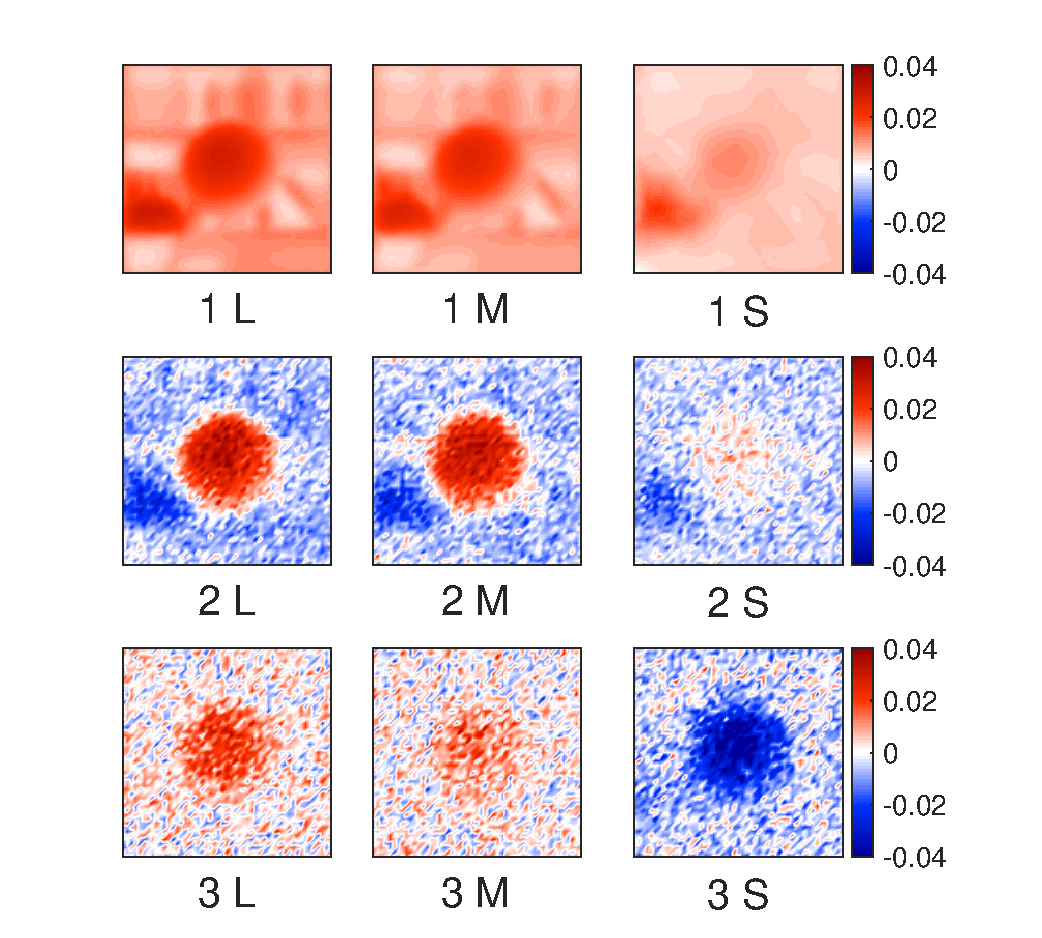
\includegraphics[width=1.0\textwidth, trim={0.2cm -0.cm 0 0.3cm}]{../FiguresDraft5/FigureSI/SI_Figure1_a.pdf}
	\label{fig:case1RFs}
    \end{subfigure}   
    \begin{subfigure}[b]{0.4 \textwidth}
	\caption{\DIFdelbeginFL \DIFdelFL{Normalized contrast}\DIFdelendFL \DIFaddbeginFL \DIFaddFL{Contrast normalized}\DIFaddendFL }
	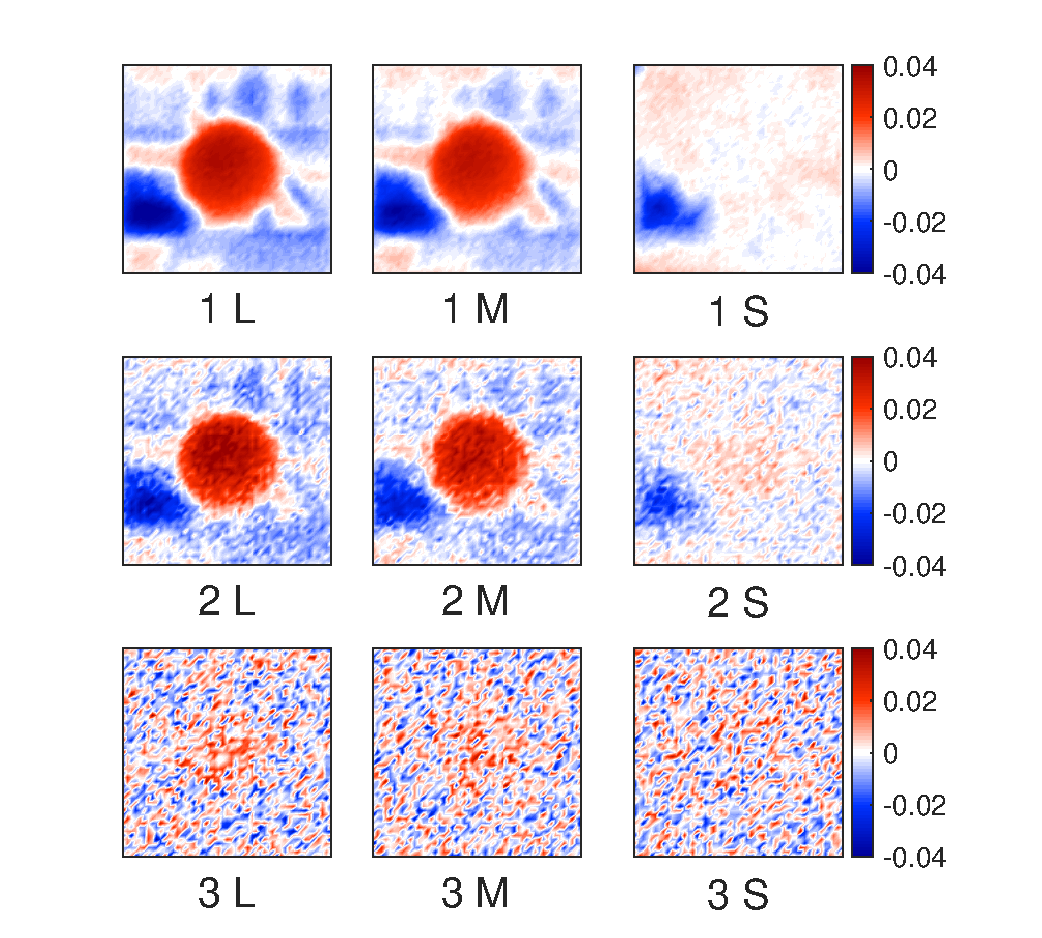
\includegraphics[width=1.0\textwidth, trim={0.2cm -0.cm 0 0.3cm}]{../FiguresDraft5/FigureSI/SI_Figure1_b.pdf}
	\label{fig:case1RFs}
    \end{subfigure}   
    \caption{{\bf Condition 2 receptive fields:} The first three AMA receptive fields learnt on (a) Cone excitations (b) \DIFdelbeginFL \DIFdelFL{Normalized contrast}\DIFdelendFL \DIFaddbeginFL \DIFaddFL{Contrast normalized}\DIFaddendFL .}
\label{fig:Condition1}
\end{figure}




\bibliography{references}

\end{document}
